\documentclass[10pt]{article}

%Math
\usepackage{amsmath}
\usepackage{amsfonts}
\usepackage{amssymb}
\usepackage{amsthm}
\usepackage{ulem}
\usepackage{stmaryrd} %f\UTF{00FC}r Blitz!
\usepackage{tikz}

\usepackage{multirow}
\usepackage{multicol}
\usepackage{tikz}
\usetikzlibrary{shapes,arrows}

%PageStyle
\usepackage[ngerman]{babel} % deutsche Silbentrennung
\usepackage[utf8]{inputenc} 
\usepackage{fancyhdr, graphicx}
\usepackage[scaled=0.92]{helvet}
\usepackage{enumitem}
\usepackage{parskip}
\usepackage[a4paper,top=2cm]{geometry}
\setlength{\textwidth}{17cm}
\setlength{\oddsidemargin}{-0.5cm}


%My Commands
\newcommand{\RN}{\mathbb{R}} %Real Number
\newcommand{\NN}{\mathbb{N}} %Natural Number
\newcommand{\QN}{\mathbb{Q}} %Rational Number
\newcommand{\ZN}{\mathbb{Z}} %ganze Zahlen
\newcommand{\CN}{\mathbb{C}} %Komplexi Zahle lawl
\newcommand{\PN}{\mathbb{P}} %Primzahle Bitches
\newcommand{\Teilt}{\mid} %|
\newcommand{\Teiltn}{\nmid} %kein teiler
\newcommand{\Potp}{\mathcal{P}} %Potenzmenge
\newcommand{\Pota}{\mathcal{A}}
\newcommand{\Potr}{\mathcal{R}}
\newcommand{\Potn}{\mathcal{N}}
\newcommand{\Bold}[1]{\textbf{#1}} %Boldface
\newcommand{\Kursiv}[1]{\textit{#1}} %Italic
\newcommand{\T}[1]{\text{#1}} %Textmode
\newcommand{\Nicht}[1]{\T{\sout{$ #1 $}}} %Streicht Shit durch
\newcommand{\lra}{\leftrightarrow} %Arrows
\newcommand{\ra}{\rightarrow}
\newcommand{\la}{\leftarrow}
\newcommand{\lral}{\longleftrightarrow}
\newcommand{\ral}{\longrightarrow}
\newcommand{\lal}{\longleftarrow}
\newcommand{\Lra}{\Leftrightarrow}
\newcommand{\Ra}{\Rightarrow}
\newcommand{\La}{\Leftarrow}
\newcommand{\Lral}{\Longleftrightarrow}
\newcommand{\Ral}{\Longrightarrow}
\newcommand{\Lal}{\Longleftarrow}
\newcommand{\Vektor}[1]{\vec{#1}}
\newcommand{\Brace}[1]{\left( #1 \right)} %()
\newcommand{\Bracel}[1]{\left\lbrace #1 \right.} %(
\newcommand{\Bracer}[1]{\right. #1 \right\rbrace} %)
\newcommand{\Brack}[1]{\left\lbrace #1 \right\rbrace} %{}
\newcommand{\Brackl}[1]{\left\lbrace #1 \right.} %{
\newcommand{\Brackr}[1]{\right. #1 \right\rbrace} %}
\newcommand{\Result}[1]{\underline{\underline{#1}}} %Doppelt unterstrichen
\newcommand{\Abs}[1]{\left| #1 \right|} %Absolutbetrag
\newcommand{\Norm}[1]{\Abs{\Abs{ #1 }}} %Norm
\newcommand{\Arrays}[1]{\left(\begin{array}{c}#1\end{array}\right)} %Array mit einer Kolonne ()
\newcommand{\Array}[2]{\left(\begin{array}{#1}#2\end{array}\right)} %Array mit n Kolonnen ()
\newcommand{\Bracka}[2]{\left\lbrace\begin{array}{#1}#2\end{array}\right\rbrace} %Array mit {}
\newcommand{\Brackal}[2]{\left\lbrace\begin{array}{#1} #2 \end{array}\right.} %Array mit {
\newcommand{\Brackar}[2]{\left.\begin{array}{#1} #2 \end{array}\right\rbrace} %Array mit }
\newcommand{\Sumone}[2]{\sum_{#2=1}^{#1}} %Summe von 1
\newcommand{\Sumz}[2]{\sum_{#2=0}^{#1}} %Summe von 0
\newcommand{\Sum}[2]{\sum_{#2}^{#1}} %Allgemeine Summe
\newcommand{\Oneover}[1]{\frac{1}{#1}} %1 über igendwas
\newcommand{\Tablewt}[3]{\begin{table*}[h]\caption{#1} \begin{tabular}{#2}{#3}\end{tabular}\end{table*}} %Table mit Titel
\newcommand{\Oben}[2]{\overset{#1}{#2}} %etwas über etwas anderem
\newcommand{\Unten}[2]{\underset{#1}{#2}} %etwas unter etwas anderem
\newcommand{\Bildcap}[2]{\begin{figure}[htb]\centering\includegraphics[width=0.2\textwidth]{#1} \caption{#2}\end{figure}} %Bild mit beschriftung
\newcommand{\Bildjpeg}[1]{\includegraphics[width=0.2\textwidth]{#1.jpeg}} %Bilder jpeg!!
\newcommand{\Bildjpg}[1]{\includegraphics[width=0.2\textwidth]{#1.jpg}} %Bilder jpg!!
\newcommand{\Bild}[1]{\includegraphics[width=0.4\textwidth]{#1}} %Bilder jpg!!
%Beispiel für lstlisting \lstinputlisting[label=Aufgabe 4a,caption=Aufgabe 4a]{4a.java}

% Code listenings
\usepackage{color}
\usepackage{xcolor}
\usepackage{listings}
\usepackage{caption}
\DeclareCaptionFont{white}{\color{white}}
\DeclareCaptionFormat{listing}{\colorbox{gray}{\parbox{\textwidth}{#1#2#3}}}
\captionsetup[lstlisting]{format=listing,labelfont=white,textfont=white}
\lstdefinestyle{JavaStyle}{
 language=Java,
 basicstyle=\footnotesize\ttfamily, % Standardschrift
 numbers=left,               % Ort der Zeilennummern
 numberstyle=\tiny,          % Stil der Zeilennummern
 stepnumber=5,              % Abstand zwischen den Zeilennummern
 numbersep=5pt,              % Abstand der Nummern zum Text
 tabsize=2,                  % Groesse von Tabs
 extendedchars=true,         %
 breaklines=true,            % Zeilen werden Umgebrochen
 frame=b,         
 %commentstyle=\itshape\color{LightLime}, Was isch das? O_o
 %keywordstyle=\bfseries\color{DarkPurple}, und das O_o
 basicstyle=\footnotesize\ttfamily,
 stringstyle=\color[RGB]{42,0,255}\ttfamily, % Farbe der String
 keywordstyle=\color[RGB]{127,0,85}\ttfamily, % Farbe der Keywords
 commentstyle=\color[RGB]{63,127,95}\ttfamily, % Farbe des Kommentars
 showspaces=false,           % Leerzeichen anzeigen ?
 showtabs=false,             % Tabs anzeigen ?
 xleftmargin=17pt,
 framexleftmargin=17pt,
 framexrightmargin=5pt,
 framexbottommargin=4pt,
 showstringspaces=false      % Leerzeichen in Strings anzeigen ?        
}

\tikzstyle{decision} = [diamond, draw, fill=blue!20,
   text width=5.8em, text badly centered, node distance=3.5cm, inner sep=0pt]
\tikzstyle{block} = [rectangle, draw, fill=blue!20,
   text width=5em, text centered, rounded corners, minimum height=4em]
\tikzstyle{line} = [draw, very thick, color=black!50, -latex']
\tikzstyle{cloud} = [draw, ellipse,fill=red!20, node distance=2.5cm,
   minimum height=2em]

%Config
\renewcommand{\headrulewidth}{0pt}
\setlength{\headheight}{15.2pt}

%Metadata
\title{
	\vspace{5cm}
	Kryptographie
}
\author{Fabio Oesch,  Michael Künzli \& Jan Fässler}
\date{4. Semester (FS 2013)}


% hier beginnt das Dokument
\begin{document}

% Titelbild
\maketitle
\thispagestyle{fancy}

\newpage

% Inhaltsverzeichnis
\pagenumbering{Roman}
\tableofcontents	  	


\newpage
\setcounter{page}{1}
\pagenumbering{arabic}

\section{Mathematische Grundlagen}
\subsection{Grundlagen}
\subsubsection{Einwegfunktion}
In der Informatik ist eine Einwegfunktion eine mathematische Funktion, die komplexitätstheoretisch „leicht“ berechenbar, aber „schwer“ umzukehren ist. 
\subsubsection{Eigenschaften Funkionen}
\begin{description}
\item [Injektiv] Jedes x hat sein eigenes y.
\item [Surjektiv] Wenn das Bild der Wertemenge entspricht.
\item [Bijektiv] Wenn Injektiv wie Surjektiv 
\end{description}
\subsubsection{Kombinatorik}
$\binom{n}{k} = \frac{n!}{k!(n-k)!}$
\subsubsection{(erweiterter) Euklid}
\textbf{ggT(a,b):} \\
$a=q*b+b_{neu}$ \hspace*{1cm} $s_1=1$ \& $t_1=0$ \hspace*{0.75cm} $s=t_{\T{alt}}$ \& $t=s_{\T{alt}}-q\cdot t_{\T{alt}}$\\
\begin{tabular}{| c | c | c | c | c |}
   \hline
   $a$ & $b$ & $q$ & $s$ & $t$ \\
   \hline
   99 & 78 & 1 &  & \\
   78 & 21 & 3 &  & \\
   21 & 15 & 1 &  & \\
   15 & 6 & 2 &  & \\
   6 & 3 & 2 &  & \\
   3 & 0 &  &  & \\\hline
\end{tabular}
\begin{tabular}{| c | c | c | c | c |}
   \hline
   $a$ & $b$ & $q$ & $s$ & $t$ \\
   \hline
   99 & 78 & 1 &  & \\
   78 & 21 & 3 &  & \\
   21 & 15 & 1 &  & \\
   15 & 6 & 2 &  & \\
   6 & 3 & 2 &  & \\
   3 & 0 &  & 1 & 0 \\\hline
\end{tabular}
\begin{tabular}{| c | c | c | c | c |}
   \hline
   $a$ & $b$ & $q$ & $s$ & $t$ \\
   \hline
   99 & 78 & 1 & -11 & 14\\
   78 & 21 & 3 & 3 & -11\\
   21 & 15 & 1 & -2 & 3\\
   15 & 6 & 2 & 1 & -2\\
   6 & 3 & 2 & 0 & 1\\
   3 & 0 &  & 1 & 0 \\\hline
\end{tabular}\\
\\
Daraus folgt dann $3=-11\cdot99+14\cdot78$
\subsubsection{Diophantische Gleichungen}
Die Gleichung $ax + by = c$ ist eine diophantische Gleichung. Sie besitzt nur eine ganzahlige Lösung, wenn $ggT(a, b)\|c$. Gibt es eine Lösung, gibt es unendlich viele Lösungen. Eine mögliche Lösung kann mit dem erweiterten euklidischen Algo. gefunden werden. Soll x oder y in einem bestimmten Bereich liegen, kann man sie mit folgender Formel shiften: $c = ax + by$, $0 = kab - kab$ addiert: $c = ax + kab + by - kab$, $c = a(x + kb) + b(y - ka)$
\subsection{Modulares Rechnen}
\subsubsection{Division}
Eine modulare Division hat die Form \fbox{$a/b$ mod $n$} , gesucht wird die ganze Zahl $c$ im Intervall $[0,n-1]$, welche die Gleichung \fbox{$bc\equiv a$ mod $n$}. Die modulare Division ist nur möglich, wenn $ggT(b,n)=1$. \\
\\
\textbf{Beispiel}: $23/27$ mod $31$ {\color{gray} // wenn ($ggT(27,31) = 1 \rightarrow$  modulare Division möglich) }\\
erweiterten euklidischen Algorithmus: $23 * \textbf{7} * 31 + 23 * \textbf{(-8)} * {\color{red}27}$  {\color{gray}// erweitern mit 23}\\
\\
$\Longrightarrow$ Uns interessiert nur $c = 23 * (-8) = -184$ was der \textbf{Restklasse 2} (von Modulo 31) entspricht. Dies ermittelt man, indem man zu -184 so oft 31 addiert, bis man eine positive Zahl erhält. Die gesuchte Gleichung lautet also: $27 * 2 \equiv 23$ mod $31$.
\subsubsection{Potenzieren}
Seien $a,b,n \in \ZN$ und $b,n > 1$. Berechnen Sie $a^b$ mod $n$.
\begin{itemize}
	\item[1.)] binäre Darstellung von b: $b=\sum_{i=0}^k \alpha_i2^i$ mit $\alpha \in \{0,1\}$.
	\item[2.)] Anwendung auf a: \\
		$a^{\sum_{i=0}^k \alpha_i2^i}$ = $\prod_{i=0}^{k} a^{\alpha_i2^i}$ = $a^{\alpha_k2^k}*a^{\alpha_{k-1}2^{k-1}}*a^{\alpha_{k-2}2^{k-2}} \dots  a^{\alpha_12}*a^{\alpha_0}$ = $($\dots$((a^{a_k})^2*a^{a_{k-1}})^2$\dots$*a^{\alpha_1})^2*a^{\alpha_0}$
	\item[3.)] Das Verfahren besteht nun darin, den letzten Ausdruck von innen nach aussen auszuwerten und nach jeder Multiplikation das Resultat modulo $n$ zu rechnen.
\end{itemize}
\textbf{Beispiel:}  $977^{2222}$ mod $11$
\begin{itemize}
	\item[1.)] $2222_{10} \blacktriangleright$ bin $= 100010101110_2$
	\item[2.)] ( \dots $ (977)^2)^2)^2)^2*977)^2)^2*977)^2)^2*977)^2*977)^2*977)^2 {\color{gray} *(0*977)}$
	\item[3.)] Anwendung des Verfahren: \\
	\begin{tabular}{l l l p{3cm} l l l}
	 977 & mod 11 & = 9     & $5^2$ & mod 11 & = 3 \\
	 $9^2$ & mod 11 & = 4   && $3^2$ & mod 11 & = 9 \\
	 $4^2$ & mod 11 & = 5   && $9*977$ & mod 11 & = 4 \\
	 $5^2$ & mod 11 & = 3   && $4^2$ & mod 11 & = 5 \\
	 $3^2$ & mod 11 & = 9   && $5*977$ & mod 11 & = 1 \\
	 $9*977$ & mod 11 & = 4 && $1^2$ & mod 11 & = 1 \\
	 $4^2$ & mod 11 & = 5   && $1*977$ & mod 11 & = 9 \\
	 $5^2$ & mod 11 & = 3   && $9^2$ & mod 11 & = \textbf{4} \\
	 $3*977$ & mod 11 & = 5\\

	\end{tabular}
\end{itemize}
\subsubsection{Chinesischer Restsatz}
 $x\equiv {\color{blue}m_1}\T{ mod }{\color{purple}n_1}$ \\
 $x\equiv {\color{blue}m_2}\T{ mod }{\color{purple}n_2}$\\
 $x\equiv {\color{blue}m_3}\T{ mod }{\color{purple}n_3}$\\
\\
$N={\color{purple}n_1\cdot n_2 \cdot n_3}$, 
${\color{brown}N_i}=\frac{N}{\color{purple}n_i}$\\
\\
$ggT({\color{brown}N_i},{\color{purple}n_i})=x\cdot {\color{purple}n_i}+y\cdot {\color{brown}N_i} = 1 \to {\color{red}e_i}=y\cdot {\color{brown}N_i}$ \hspace{1cm}{\color{gray}// erweiterter Euklid}\\
 \\
 $x={\color{blue}m_1}\cdot {\color{red}e_1}+{\color{blue}m_2}\cdot {\color{red}e_2}+{\color{blue}m_3}\cdot {\color{red}e_3}\T{ mod } N$ 
 
\subsection{Kettenbruch}
$x=a_0+\frac{1}{a_1+\frac{1}{a_2+\frac{1}{\quad\stackrel{\vdots}{a_{n-1}+\frac{1}{a_n}}}}}$. Für diesen Ausdruck schreiben wir auch: $<a_0;a_1,a_2,a_3,\ldots,a_n>$ \\
Berechnen mittels Euklid. Bsp: $\frac{37}{7}$ $\rightarrow$ $\text{ggt}(37, 7)$\\
$37 = \textbf{5}*7 + 2$\\
$7 = \textbf{3}*2 + 1$\\
$2 = \textbf{2}*1 + 0$ $\rightarrow$ $<5;3,2>$ \\
\\
Sei: $\alpha \in \mathbb{Q} \backslash \mathbb{Z}$ dann sei $<x_0; x_1, x_2, \ldots, x_n>$ Approximation von $\alpha$.

\subsection{Gruppen}
\subsubsection{Notation}
Eine Gruppe ist ein Tripel $(G, *, e)$. $G$ ist eine Menge, $*$ eine Binärverknüpfung und $e$ ein ausgezeichnetes Element der Menge $G$. Das Tripel muss folgende Eigenschaften erfüllen um eine Gruppe zu sein:
\begin{enumerate}
	\item Assozivität: $\forall a,b,c \in G : f(f(a,b),c) = f(a,f(b,c))$
	\item Neutrales Element: $\forall a \in G : f(a,e) = f(e,a) = a$
	\item Inverses Element: $\forall a \in G:\exists b \in G:f(a,b)=e$
\end{enumerate}
Die Abbildung $f$ ist die Vorhinbezeichnete Abbildung $*$ zwischen den Mengen. Ist Gruppe zu dem noch Kommutativ, ist es eine abelsche Gruppe: $\forall a, b \in G : a * b = b * a$
\subsubsection{Spezielle Mengen}
Die Menge $\ZN^*_n$ ist definiert als: $\{a \in \ZN_n|ggT(a,n,=)1\}$.
\subsubsection{Ordnung der Gruppe}
Die Anzahl der Elemente in der Gruppe wird Ordnung genannt. Für eine Gruppe $\ZN^*_n$ gilt $\phi(n)$
\subsubsection{Erzeugende Elemente, zyklische Gruppen}
Die Menge $<a>$ ist definiert als: $<a>:= \{an|n \in \ZN\}$. Enthält die daraus erzeugte Menge aller Elemente der Gruppe, so wird die Gruppe als zyklisch bezeichnet. Zusätzlich wird definiert das $a^0 = e$ und $a^{-1} =$ invereses von $a$.
\subsubsection{Gruppenhomomorphismus}
Der Gruppenhomomorphismus ist eine strukturerhaltenden Abbildung. Seien $(G,\bullet,e_g)$ und $(H,\bullet,e_h)$. Das heisst, es gibt eine Abbildung $f$ für die gilt: $f(x*y) = f(x) \bullet f(y)$. Das neutrale Element muss immer auf das neutrale Element der anderen Gruppe abgebildet werden!
\subsubsection{Satz Euler Fermart}
Der Satz lautet: $a^{\phi(n)} = 1\T{ mod }n$
\subsection{Faktorisierung}
\subsubsection{Fermat}
$n=ab$, $n$ soll faktorisiert werden. 
\begin{enumerate}
\item $t = \lfloor \sqrt n \rfloor + 1$. 
\item Wenn $t^2 - n$ ein Quadrat weiter bei 4.
\item $t = t + 1$ Weiter bei 2.
\item $s := \sqrt{t^2 -n}, a = t + s, b = t - s$
\end{enumerate}
Bemerkung: Der Alog terminiert immer, da gilt: $t \le \frac{n+1}{2}$
Aufwand: $\frac{c^2}{8}$ und $c$ ist eine geeignete Konstante. $\Delta := p-q < c \sqrt[4]{n}$ {\color{red} $\Ra$ Resultat ist unabhängig von n!!!} 

\subsubsection{Polard $p -1$}
\begin{enumerate}
\item Alle Primzahlen $q$ mit $q \le B$
\item $\beta(q, B) = \text{max}\{B \in \mathbb{N}: q^\beta \le B\}$
\end{enumerate}
Beispiel:
$n=1241143$, $B=13$ Das $B$ ist willkürlich gewählt. $a$ wählen: $ 1 < a < n$ und $ggT(a, n)$ $= 1$. \\
Menge bilden: ${2, 3, 5, 7, 11, 13}$ ($\forall$ $\PN<=B$). Nun alle Exponenten suchen: $\beta (2, 13) = 3$, da $2^3 < 13$. Dann $\beta (3, 13) = 2)$, 
$\beta (5, 13) = \beta (7, 13) = \beta (11, 13) = \beta (13, 13) = 1$ \\
$k = 2^3 * 3^2 * 5 * 7 * 11 * 13$ einsetzen in $ggT(a^k-1, n)$ $= 557 \in \PN$

\newpage
\section{Definition eines Kryptosystems}
\subsection{Passiver Angreifer}
Einer, der nur mithört.
\subsection{Prinzip von Kerkhoffs}
\begin{itemize}
	\item Trennung von Verschlüsselungsmaschine und Schlüssel
	\item Die Verschlüsselungsmaschine ist dem Gegner bekannt
	\item Das zu schützende Geheimnis ist der Schlüssel
\end{itemize}
\subsection{Formale Beschreibung Kryptosystems}
System: $(P, C, K, e, d)$, $P$ Menge der Klartexte, $C$ Menger der Geheimtexte, $K$ Menge der Schlüssel:
$e: K \times P \rightarrow C$; $d: K \times C \rightarrow P$
Es gilt: $\forall k \in K \forall p \in P: d (k, e (k, p)) = p$ $\implies$ $\forall k \in K : e(k, -)$ ist injektiv; $\forall k \in K: d(k, -)$ ist surjektiv.
\subsection{Attacken auf Kryptosystem}
\begin{enumerate}
\item \textbf{Ciphertext-onlyattack} \\
Gegeben $c_i= ek(p_i)$ , i = 1, ... , n \\
Gesucht: $p_i$, i = 1, ... , n oder k
\item \textbf{Known-plaintextattack}\\
Gegeben $( p_i, c_i= ek(p_i))$ , i = 1, ... , n \\
Gesucht: k 
\item \textbf{Chosen-plaintextattack}\\
Gegeben: $( p_i, c_i= ek(p_i))$ , i = 1, ... , n \\
pinach Wahl des Kryptoanalytikers \\
Gesucht: k 
\item \textbf{Chosen-ciphertextattack}\\
Gegeben: $( c_i,p_i= dk(c_i))$ , i = 1, ... , n \\
$c_i$ nach Wahl des Kryptoanalytikers \\
Gesucht: k
\end{enumerate}

\newpage
\section{Klassische Kryptographie}
\subsection{Klassen}
\begin{tabular}{l | l}
	\textbf{Substitution Cipher} & \textbf{Transposition Cipher} \\
	\hline \\
	Einheiten werden \textbf{ersetzt}. & Einheiten werden \textbf{vertauscht}. \\
	& \begin{tabular}{c c c c c c}
		3 & 1 & 5 & 6 & 2 & 4 \\\hline
		K & O & M & M & E & H \\
		E & U & T & E & A & B \\
		E & N & D & Z & U & M \\
		Z & O & O & A & B & C \\
	\end{tabular} \\
	& $\Ra \underbrace{\T{OUNO}}_1\underbrace{\T{EAUB}}_2\dots$ \Bold{Bem.}\\
	&  Einheiten werden vertauscht\\
	& (ABC ist Padding)
\end{tabular} \\ \\

\begin{tabular}{l|l}
 \Bold{monoalphabetisch}&\Bold{polyalphabetisch}\\
 $E:\Pota\ra B$, $x\mapsto E(x)$&$E:\Pota\ra P(B)$, $x\mapsto E(x)$\\\hline
 \Bold{monographisch}&\Bold{polygraphisch}\\
 Buchstaben&Gruppen von Buchstaben
\end{tabular}

\subsection{Caesar Cipher}
Einfacher substitions Cipher bei welchem das Alphabet ``verschoben'' wird. Beispiel: A B \ldots Z $\rightarrow$ B C \ldots A. Sei $ord(c)$ eine Funktion, welche jedem Buchstaben einen numerischen Wert zuweise. Beispiel: $ord(a) = 0, ord(b) = 1$ etc. Weiter sei offset der Wert um welchen verschoeben werden soll. So kann mit $ord(\text{mc}) + offset \mod 26$ der Index des Buchstabens der Geheimnachricht bestummen berechnet. Auf gleiche Weise lässt sich ein Text entschlüsseln.

\subsubsection{Attacken}
Mit dem Wissen, in welcher Sprache die Nachricht geschrieben wurde, lässt sich mittels Häufigkeitsanalysen die Verschiebung bestimmen. Zum Beispiel ist das ``e'' in der deutschen Sprache ein sehr häufiger Buchstabe. Wird in der Geheimnachricht gleich häufig wie ein ``e'' zum Beispiel ein ``i'' entdeckt, kann die Verschiebung bestimmt werden.

\subsection{Kasiski-Text (monographisch \& polyalphabetisch)}
\begin{description}
	\item[Klartext] TO BE OR NOT TO BE
	\item[Schlüssel] NOW
	\item[$\mathbf{p}$] $=\Abs{\T{NOW}}$
\end{description}
\begin{tabular}{c|c|c|c|c}
 TOB&EOR&NOT&TOB&E\\
 NOW&NOW&NOW&NOW&N\\
 GCX&RCN&ACP&GCX&R
\end{tabular}\\
GCX kommt 2x for so können wir eine Annahme zur Periode $p$ machen. Die Periode ist dann $c\cdot p$. Dies kann aber auch zufällig passieren.

\subsection{Playfair}
\subsubsection{Konstruktion Playfair-Quadrat}
$\mathbf{Keyword}$ (Doppelte Streichen), dann der Rest des Alphabets ohne Buchstaben des Keywords.\\\\
$\begin{matrix}
\mathbf{D} & \mathbf{E} & \mathbf{A} & \mathbf{T} & \mathbf{H} \\
B & C & F & G & I/J \\
K & L & M & N & O \\
P & Q & R & S & U \\
V & W & X & Y & Z \\
\end{matrix}$
\subsubsection{Ver-/Entschlüsselung}
\begin{tabbing}
\hspace{16em} \= \kill
Doppelbuchstaben durch X trennen \> (PA AR $\Rightarrow$ PA XA R)\\
Klartext:  \>  LA BO UL AY EL AD YW IL LX \\
Geheimtext: \> ME IK QO TX CQ TE ZX CO MW \\
\end{tabbing}
Es werden jeweils Paare verschlüsselt.\\
(Entschlüsselung in entgegengesetzter Richtung der Verschlüsselung)\\
Wrap around and den Kanten.
\begin{multicols}{2}
\subsubsection*{Selben Zeile oder Spalte}
\begin{tabbing}
\hspace{10em} \= \kill
$\begin{matrix}
* & E & * & * & * \\
* & C & * & * & * \\
* & L & * & * & * \\
* & Q & * & * & * \\
* & * & * & * & * \\
\end{matrix}$ 
\>
$\begin{matrix}
D & E & A & T & * \\
* & * & * & * & * \\
* & * & * & * & * \\
* & * & * & * & * \\
* & * & * & * & * \\
\end{matrix}$

\\ 
$ EL \rightarrow CQ$\> $AD \rightarrow TE $ \\
1 nach unten\>1 nach rechts
\end{tabbing} 
\subsubsection*{Untersch. Zeilen bzw. Spalten}
$\begin{matrix}
* & E & A & * & * \\
* & * & * & * & * \\
* & L & M & * & * \\
* & * & * & * & * \\
* & * & * & * & * \\
\end{matrix}$\\
$LA \rightarrow ME$\\
Gleiche Zeile, Seite wechseln
\end{multicols}
\subsection{Vigenère Cipher}
Funktioniert gleich wie der caesar cipher, nur wird der Geheimtext nicht nur mit einer Verschiebung erzeugt sondern mit einem geheimen Satz (Schlüssel): Die Nachricht und der Schlüssel werden untereinander geschrieben. Dabei wird der Schlüssel solange wiederholt, bis unter jedem Buchstaben der Nachricht ein Buchstaben des Schlüssels steht. Die Buchstaben des Schlüssels geben die Verschiebung des Buchstabens der Nachricht an.
\subsubsection{Kasiski Test}
\begin{multicols}{2}
\begin{enumerate}
\item Paare von min. Länge 3 finden
\item Abstände innerhalb der Paare bestimmen
\item Abstände Faktorisieren
\item Häufigster Faktor $\Rightarrow$ Kandidat für Schlüssellänge
\end{enumerate}
\end{multicols}
\subsubsection{Koinzidenz Index}
\begin{multicols}{2}
\fbox{$\mathbf{IC_{text}} = \sum_{i=1}^n p_i^2$} \\ \\
\fbox{$\mathbf{IC_text} = \frac{\sum_{i=A}^{Z}n_i(n_i -1)}{N(N-1)}$} \\
$IC_{eng} = 0.066895$\\
$IC_{ger} = 0.076667$\\
$IC_{flat}=0.0385$\\
\end{multicols}
Gegeben: Alphabet A mit $|A|=26$ $IC_{Lang} = \Sigma_{i=1}^{26} p_i^2$ \\
Beispiel: Konsonanten gleiche Wahrscheinlichkeit $p$; I, O, U = doppelte Wahrscheinlichkeit $2p$; E,A = vierfache Wahrscheinlichkeit $4p$. Zusammen zählen: $21p + 3*2p + 2*4p = 35p$. Für die Formel gilt dann: $21\frac{1}{35}^2 + 3\frac{2}{35}^2 + 2\frac{4}{35}^2$
\subsubsection{Berechnung der Schlüssellänge}
Gegeben: $C$: Vigenère-Chiffrat der Länge $n$ mit der Schlüssellänge $p$.
$\gamma = \alpha IC_L + \beta IC_{flat}$ $\alpha$:Anzahl Buchstabenpaare aus der selben Spalte. $\beta$ Anzahl Buchstabenpaare aus verschiedenen Spalten. $\gamma$ Anzahl gleicher Buchstaben aus $C$. $IC$: Koinzidenzindex des Chiffrats, $IC_L$ Koinzidenzindex der Sprache.\\
Formel: $p = \frac{n * (IC_L - IC_{Flat})}{IC(n-1) + IC_L - n*IC_{Flat}}$
\subsection{Vigenères Chipres}
\subsubsection{Beschreibung}
Das Schlüsselwort sei „AKEY“, der Text „geheimnis“. Vier Caesar-Substitutionen verschlüsseln den Text. Die erste Substitution ist eine Caesar-Verschlüsselung mit dem Schlüssel „A“. „A“ ist der erste Buchstabe im Alphabet. Er verschiebt den ersten Buchstaben des zu verschlüsselnden Textes, das „g“, um 0 Stellen, es bleibt „G“. Der zweite Buchstabe des Schlüssels, das „K“, ist der elfte Buchstabe im Alphabet, er verschiebt das zweite Zeichen des Textes, das „e“, um zehn Zeichen. Aus „e“ wird ein „O“ (siehe Tabelle). Das dritte Zeichen des Schlüssels („E“) verschiebt um 4, „Y“ um 24 Stellen. Die Verschiebung des nächsten Buchstabens des Textes beginnt wieder bei „A“, dem ersten Buchstaben des Schlüssels: \\ \\
\begin{tabular}{l c c c c c c c c c }
	\textbf{Klartext}: & g & e & h & e & i & m & n & i & s \\
	\textbf{Schlüssel}: & A & K & E & Y & A & K & E & Y & A \\
	\textbf{Geheimtext}: & G & O & L & C & I & W & R & G & S 
\end{tabular}
\subsubsection{Kryptoanalysis des Vigen\`{e}re-Cipher}
\begin{description}
	\item[1)] Schlüssellänge p=1,2,3,\dots
		\begin{itemize}
			\item Einleitung des Cipher-Tests in p Abschnitte
			\item Berechnung des IC des Abschnitts
			\item Wähle p mit $IC\sim IC_L$ (oder hoch)
		\end{itemize}
	\item[2)] Sei s,t zwei  Strings über dem Alphabet A: $s=s_1,s_2,s_3,$ \dots$. s_k$ / $t=t_1,t_2,t_3,$ \dots$, t_l$ \\
		Seien $n_1(s) :=$ \#A's in s, $n_2(s) :=$ \#B's in s, \dots
	\item[Def.] $MIC(s,t):=\frac{\sum_{i=1}^{26}n_i(s)*n_i(t)}{k*l}$
	\item[Beispiel:] s="{}AABCCA" / t="{}ABCABCABC" \\
		$\Brackar{l}{ n_1(s)=3, n_1(t)=3 \\ n_2(s)=1, n_2(t)=3 \\ n_3(s)=2, n_3(t)=3} \ra$ $MIC(s,t)=\frac{1}{6*9}[3*3+1*3+2*3]$

	\item[3.)] \textbf{Anwendung auf Cipher Text} \\
		\begin{tabular}{l l}
			\multirow{6}{*}{
			\begin{tabular}{|c|c|c|c|c|}\hline
				$(i,j)\backslash k$&0&1&2&$\cdots$\\\hline
				$(1,2)$&&&&\\
				$(1,3)$&&&&\\
				$(1,4)$&&&&\\
				$(1,5)$&&&&\\\hline
				$(2,3)$&&&$MIC(c_2,c_{3+2})$&\\\hline
				$(2	,4)$&&&&\\
				$(2,5)$&&&&\\
				$(3,4)$&&&&\\
				$(3,5)$&&&&\\
				$(4,5)$&&&&\\\hline
			\end{tabular}
			} & p = Schlüssellänge von c (Annahme:5) \\
			& $c_1,c_2, ...,c_5$ Abschnitte des Ciphertext \\
			& $i=1,$ \dots$,p$ \\
			& $j=i+1,$ \dots$,p$ \\
			& $k=0,$ \dots$,25$ \\
			& $\to MIC(c_i,c_{j+k})$ \\
			& \\
			& Beispiel: \\
			& $c_1$:AXBM\dots\\
			& $c_3$:ABXH\dots \\
			& $------$ \\
			& $c_{3+2}$:CDZJ\dots \\
		\end{tabular} \\

	\item[4.)] Wir suchen Einträge in der Tabelle, die hoch sind ($> 0.06$) \\
		$MIC(s,t)=\Oneover{kl}\Sum{26}{i=1}n_i(s)n_i(t)$, $\Abs{s}=k$, $\Abs{t}=l$\\
		zb: $MIC(c_2,c_3{+22} > 0.06 \Longleftrightarrow c_2 \sim c_3+22 \Ra$\fbox{$\beta_2-\beta_3=k$} \\
	\item[Notation] s$\sim$t $\Longleftrightarrow$ s und t sind mit dem gleichen Shift aus zwei Klartexten entstanden.
	\item[Bsp.] $klar_1 \sim klar_2$ \\
		\begin{tabular}{l | l | l}
			$klar_1 \xrightarrow[]{\beta_1} c_1$ & $c_1 = klar_1+\beta_1$ & ${\color{red}\beta_1}+klar_1=c_1-\beta_1+{\color{red}\beta_1}=c_1$ \\
			$klar_2 \xrightarrow[]{\beta_2} c_2$ & $c_2 = klar_2+\beta_2$ & ${\color{red}\beta_1}+klar_2=c_2-\beta_2+{\color{red}\beta_1}=c_2+(\beta_1+\beta_2)$\\
		\end{tabular} \\ \\ \\
		Wir suchen die grossen Werte von $MIC(c_i, c_j +k)$ \\
		$MIC(c_i, c_j +k)$ gross $\Longleftrightarrow$ $c_i \sim c_j + k$ \\ \\
		$c_i=klar_i+\beta_i$ $\sim$ $klar_i + \beta_j + k$ = {\color{red} $k = \beta_i + \beta_j$ }\\
		
		\hspace*{.2cm}$\downarrow$ sind \underline{bekannt}\\
		$\Brackar{c}{
		k_{12}=\beta_2-\beta_1\\
		k_{13}=\beta_3-\beta_1\\
		k_{52}=\beta_2-\beta_5\\
		}$Auflösen nach $\beta_1$\\\\
		\textbf{Schlüsselwort}: $\beta_1,\Oben{\T{abhängig von }\beta_1}{\beta_2,\dots,\beta_p}=\beta_1,\beta_1+k_{12},\dots,$ \\ 
		\textbf{Ausprobieren}: $\beta_1 = 0,1,\dots, 25$

\end{description}
\subsection{One-Time-Pad}
$\Sigma=\{0,1\}$
\begin{tabular}{lc|c|l}\cline{3-3}
Klartext:& $p_1p_2p_3p_4p_5\dots=$&$0$&$0101\dots$\\
Schlüssel:& $k_1k_2k_3k_4k_5\dots=$&$1$&$0110\dots$\\
ciphertext:& $\Unten{p_1\oplus k_1}{c_1}c_2c_3c_4c_5\dots=$&$1$&$0011\dots$\\\cline{3-3}
\end{tabular} \\
One-Time-Pad gilt als sicher, da es zu einem Ciphertext mehr als nur eine verständliche Nachricht gibt. Der Angreifer kann nicht entscheiden, welcher mögliche Schlüssel nun der richtige ist, vorausgesetzt, der Schlüssel ist solange wie die Nachricht selbst und wurde zufällig erzeugt.

\newpage
\section{Block-Cipher}
Definition Block-Cipher: $C: K \rightarrow Perm(\Sigma^n)$. $K$ ist der Schlüsselraum. $\Sigma$ = Alphabet.\\
Maximale Grösse Schlüsselraum: $|\Sigma|^n!$ wobei $n = $ Schlüssellänge. 
\subsection{Data Encription Standard (DES)}
Die Schlüssellänge von DES beträgt $56$.
\begin{tabular}{l | l l}
	\multirow{4}{*}{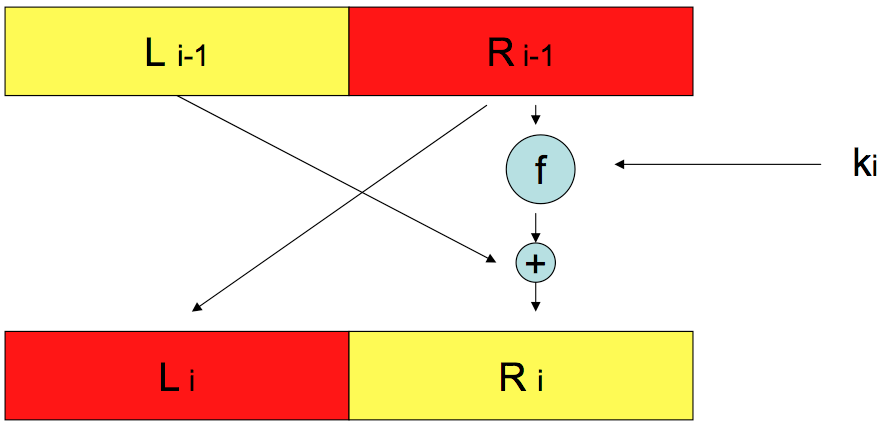
\includegraphics[scale=0.12]{horst-feistel.png}} & $L_1$ & $:= R_0$ \\
	&$R_1$ & $:= f(R_0,k_1) \oplus L_0$ \\
	&$L_0$ & $:= f(L_1,k_1) \oplus R_1$ \\
	&$R_0$ & $:= L_1$ \\
\end{tabular} \\
\subsection{Betriebsmodi}
\subsubsection{ECB-Modus (electronic code block)}
Abarbeiten der Blöcke ohne spezielles Verfahren {\color{gray} // \Bold{Bem:} $m_1=m_3\Ra c_1=c_3$} \\
 $m=\underbrace{1100}_{m_1}|\underbrace{0110}_{m_2}|\underbrace{1100}_{m_3}|101^*$ $\Unten{m_1}{\longrightarrow}$\fbox{$e_k$}$\Unten{c_1}{\longrightarrow}$ 
\subsubsection{CBC-Modus (cipher block chaining)}
\begin{tabular}{p{7.5cm}  l}
	$m=\Unten{\T{Länge n}}{m_1}|m_2|\dots$, $n:$ Blocklänge &\Bold{Bsp:} $m=\underbrace{1100}_{m_1} | \underbrace{0110}_{m_2} | \underbrace{1100}_{m_3} | 101$ \\
	{\color{red}IV = Initialvektor} (i.a. bekannt) &  $\color{red}IV=C_0=1110$  \\
	$C_0 := IV$ & $c_1 = e_k(c_0 \oplus m_1) = e_k(0010) = 0001$ \\
	$C_1 := e_k(C_0 \oplus m_1)$ & $c_2 = e_k(c_1 \oplus m_2) = e_k(0111) = 1011$ \\
	$C_2 := e_k(C_1 \oplus m_2)$  & $c_3 = e_k(c_2 \oplus m_3) = e_k(0111) = 1011$ \\
\end{tabular} \\ \\ \\
 \textbf{Entschlüsselung}:  \\
 ${\color{red}c_1\oplus} d_k(c_2)={\color{red}c_1\oplus}d_k(e_k(c_1\oplus m_2))= c_1\oplus m_2 {\color{red}\oplus c_1 = m_2}$ \\
 $m=\Unten{\T{Länge n}}{m_1}|m_2$, $n:$ Blocklänge / $IV=$Initialvektor (i.a. bekannt)\\
 $c_0:=IV$, $c_1:=e_k(c_0\oplus m_1)$, $c_2:=e_k(c_1\oplus m_2)$\\
 $c_1\oplus d_k(c_2)=d_k(e_k(c_1\oplus m_2))=c_1\oplus m_2\oplus c_1=m_2$ \\
 \Bold{Bem:} $m_1=m_3\nRightarrow c_1=c_3$\\
 \Bold{Bem:} Wenn ein C-Block korrupt ist, ist der M-Block und der danach folgende auch korrupt, alle anderen aber wieder richtig.
\subsubsection{CFB-Modus (cipher feedback)}
 $m=\underbrace{\tilde{m_1}}_{\T{Länge}=r}|\tilde{m_2}|\tilde{m_3}|\dots$, $n$: Cipher Block-Länge (DES: 64) und \fbox{$0<r\leq n$}
\begin{multicols}{2}
\subsubsection*{Modus}
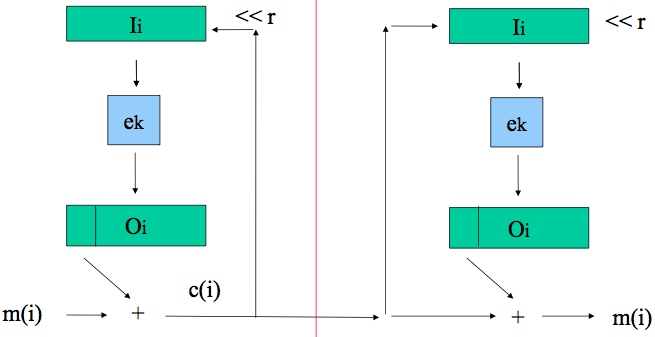
\includegraphics[scale=0.19]{cfb-encryption.png}
\subsubsection*{Beispiel}
 \begin{tabular}{ccc|ccc}
  \multicolumn{6}{c}{$m=110|001|101|100|101$, $IV=1110$, \fbox{$r=3$, $n=4$}}\\
  $I_1=$&$1110$&&$I_2=$&$\overbrace{111\mathbf{0}}^{I_1}\overbrace{\mathbf{000}}^{c_1}$\\
  &$\downarrow$&&&$\downarrow$\\
  &\fbox{$e_k$}&&&\fbox{$e_k$}\\
  &$\downarrow$&&&$\downarrow$\\
  $O_1$&$\mathbf{110}1$&&$O_2$&$\mathbf{000}0$\\
  &$\oplus$&$\to c_1$&&$\oplus$&$\to c_2$\\
  $\tilde{m_1}=$&$110$&&$\tilde{m_2}=$&$001$
 \end{tabular}
\end{multicols} 

 \newpage
\section{RSA}
\subsection{Schlüsselerzeugung}
PK = (n,e) und SK = (n,d) 
\begin{enumerate}
	\item Wähle $p,q \in \PN :p \neq q$
	\item $n=pq$
	\item Wähle $e \in \NN^* : 1<e<\phi(n)\T{ und }ggT(e,\phi(n))=1$ {\color{gray}// $\phi(n)=(p-1)(q-1) = |\ZN^*_n|$ }
	\item Finde: $d \in \NN^* :1<d<\phi(n)\T{ und }ggT(d,\phi(n))=1$ {\color{gray}// $d:=e^{-1}$ in $\ZN^*_{\varphi(n)}$} 
\end{enumerate}
\subsection{Verschlüsselung und Entschlüsselung}
\begin{description}
	\item[encryption] : $m \longrightarrow m^e$ mod n
	\item[decyption] : $m \longrightarrow c^d$ mod n
\end{description} 
\subsection{Attacken}
\subsubsection{3 Primzahlen für zwei Schlüssel}
Der RSA Provider verwendet $p_1, q_1, p_2$ um zwei Schlüssel zu erzeugen. Es gilt: $n_a = p_1 q_1$ $n_b = p_2*q_1$ Dies impliziert: $ggt(n_a, n_b) = q_1$
\subsubsection{Gleicher Modul}
$h$ berechnen: $ h = \frac{e_b d_b - 1}{ggt(e_a, e_b d_b -1)}$. Der
Angreiffer muss nun nur noch folgende Gleichung lösen: $\alpha h + \beta e_a = 1$ $\beta$ ist die Zahl, mit welcher der Angreifer die Nachrichten von Alice entschlüsseln kann. Ist $\beta < 0$ dann muss $+h$ gerechnet werden.
\subsubsection{Hastad Attack}
\begin{tabular}{l l l l l}
    & & {\color{red} $e=3$} & & $=x$ \\
	&  & Bob $(n_1,e)$ & : {\color{red}$c_1$} & $= m^3$ mod $n_1$\\
	&$\nearrow$  \\
	Alice & $\rightarrow$ & Jon $(n_2,e)$ & : {\color{red}$c_2$} & $= m^3$ mod $n_2$\\
	& $\searrow$ \\
	& & Paul $(n_3,e)$ & : {\color{red}$c_3$} & $= m^3$ mod $n_3$
\end{tabular} \\ \\
\textbf{Chinesischer Restsatz}: $m^3= crt([m^3,m^3,m^3],[n_1,n_2,n_3])$ \\
Es benötigt so viele Gleichungen für den Restsatz wie ${\color{red}e}$ gross ist.

\subsubsection{Wiener's Angriff}
\begin{description}
 \item [Voraussetzung] \hfill
    \begin{itemize}
      \item $(n,e),(n,d)$ RSA-Schlüssel mit $n=p\cdot q$, $p<q<2p$
      \item $0<d\leqslant\Oneover{3}\sqrt[4]{n}$
    \end{itemize}
 \item [Behauptung] $\exists$ schneller Alg. zur Faktorisierung von $n$
\end{description}
Konvergenten von $\frac{e}{n} = \frac{K}{\delta}$ $\phi = \frac{e \delta_{i}-1}{K_i}$\\
Bsp: $(n,e) = (2021, 773)$, $(n,d) = (2021, ?)$\\

\begin{multicols}{2}
Kettenbruch von $\frac{e}{n}$\\
\begin{align*}
773 =& 0 * 2021 + 773 \\
2021 =& 2*773 + 475 \\
773 =& 1*475 + 298 \\
475 =& 1*298 + 177 \\
298 =& 1*177 + 121 \\
\end{align*}
Konvergenten: $0, \frac{1}{2}, \frac{1}{3}, \frac{2}{5}, \frac{4}{7}, \ldots$
\begin{align*}
\phi_1 =& \frac{e*2-1}{1} = 1545\\
\phi_2 =& \frac{e*3-1}{1} = 2318\\
\phi_3 =& \frac{e*5-1}{1} = 1932\\
\phi_4 =& \frac{e*7-1}{4} = 1352.5 \notin \mathbb{Z}\\
\end{align*}
\end{multicols}
$\frac{5}{3}=$\\
\begin{tabular}{l|c|l}\cline{2-1}
 $5=$&$1$&$\cdot3+2$\\
 $3=$&$1$&$\cdot2+1$\\
 $2=$&$2$&$\cdot1$\\\cline{2-1}
\end{tabular}\\\linebreak
{\color{red}KE von $\frac{5}{3}=<1,1,2>$}\\
$1+\frac{1}{1+\frac{1}{2}}=\frac{5}{3}$\\
\begin{description}
 \item [Voraussetzung] \hfill \\
    \begin{itemize}
      \item $(n,e),(n,d)$ RSA-Schlüssel mit $n=p\cdot q$, $p<q<2p$
      \item $0<d\leqslant\Oneover{3}\sqrt[4]{n}$
    \end{itemize}
 \item [Behauptung] $\exists$ schneller Alg. zur Faktorisierung von $n$
\end{description}
\begin{lstlisting}
 e = d.invers_mod(phi)
 con = continued_fraction_list(e/n, partial_convergents = true)
\end{lstlisting}

\subsubsection{de Wenger - Spezialfall: RSA-Schlüssel}
\Bold{Vor.}
\begin{itemize}
	\item[1.] $n=p*q$, $p,q \in \PN^*$, $p>q$ 
	\item[2.] $\delta=p-q$
\end{itemize}
\Bold{Beh.} $0 < p+q - 2 * \sqrt{n} < \frac{\delta^2}{4 * \sqrt{n}}$ \\
\Bold{Bew.}
\begin{itemize}
	\item[1.] $\delta^2= (p-q)^2=(p+q)^2-4*n=(p+q-2*\sqrt{n})(p+q+2*\sqrt{n})>0$ 
	\item[2.] $p+q-2*\sqrt{n} = \frac{\delta^2}{(p+q)+2*\sqrt{n}} < \frac{\delta^2}{2*\sqrt{n}+2*\sqrt{n}}= \frac{\delta^2}{4 * \sqrt{n}}$
\end{itemize}
\subsubsection{SK-Such-Algorithmus}
{
\textbf{Gegeben}: Bob: $(n,e)$, $(n,d)$ und Alice: $(n,d_A)$ \\
\textbf{unbekannt}: $d_A,p,q,\varphi(n)$ Finde $d_A$ \\
\textbf{Bemerkung}: \\
    Falls $c=m^{m_A}$ mod $n$ ist, gilt $m=c^{d_A}$ mod $n$ \\
    $e*d-1=k*\varphi(n)$ \\
    $h:=\frac{e*d-1}{ggT(e_A,e*d-1)}$ \hspace*{2cm}//$\varphi(n)\mid h$\\
    $h:=\frac{h}{ggT(h,e_A)}$ \\
    $e_A\cdot\alpha+h\cdot\beta=1 $ {\color{red}$\Ra d_A:=\alpha$ mod $h$}
}

\section{Signaturen}
\subsection{RSA}
Alice: $(m, h(m)) \mapsto (m, sig(h(m)))$. $d(sig_{Alice}, h(m)$ \\ Alice signiert mit: $h(m)^d_{\text{Alice}} \mod n = s$ \\
Der Empfänger prüft: $s^e \mod n$
\subsection{Das Lamport-Schema}
 \Bold{Gegeben:} Ein-weg-Funktion: $f:Y\to Z$\\
 $m=x=(x_1,x_2,\dots,x_n)$ mit $x_i\in\{0,1\}$\\
 Jedes Bit wird einzeln signiert!
 \begin{enumerate}
  \item Wähle \Bold{zufällig} Elemente aus $Y$\\
  $\Brackar{|cc|}{\hline
   y_{10}&y_{11}\\
   y_{20}&y_{21}\\
   \vdots&\vdots\\
   y_{k0}&y_{k1}\\\hline
  }$\Bold{Geheim}
  \item Berechne und publiziere: $f(y_{j,j})=:z_{j,j}$\\
  \begin{tabular}{|cc|}\hline
   $z_{10}$&$z_{11}$\\
   $z_{20}$&$z_{21}$\\
   $\vdots$&$\vdots$\\
   $z_{k0}$&$z_{k1}$\\\hline
  \end{tabular}
  \item Signieren von $x_i$: $sig(x_i)=\Brackal{c}{y_{i0}\T{, falls }x_i=0\\y_{i1}\T{, falls }x_i=1}$
 \end{enumerate}
 \Bold{Bsp:} $x=(0,0,1)$
   \begin{tabular}{|cc|}\hline
   $z_{10}$&$z_{11}$\\
   $z_{20}$&$z_{21}$\\
   $z_{30}$&$z_{31}$\\\hline
  \end{tabular}
  $sig(X)=y_{10}$, $y_{20}$, $y_{31}\Oben{f}{\to}f(y_{10})$
\subsection{El-Gamal}
Ein Signaturverfahren besteht aus $4$ Mengen: $P$ Nachrichtenmenge, $S$ Signaturmenge, $SK$ der geheime Schlüssel, $PK$ der öffentliche Schlüssel. Dazu gibt es das Signaturverfahren:
\begin{align}
sig: P \times SK \rightarrow& S \\
(m,k) \mapsto sig(m, k)
\end{align}
und ein Verifikationsverfahren: $ver: P \times S \times SK \rightarrow {0,1}$\\
\textbf{Vorgehen}:
\begin{itemize}
	\item Man wähle ein grosses $p \in \mathbb{P}$
	\item Man wähle ein Erzeugens: $\omega \in \mathbb{Z}_p^*$. $p$ und $\omega$ sind öffentlich bekannt.
	\item Jeder Teilnehmer (T) wählt zufällig $a_T < p-1 \mod p$. Diese Zahl ist der geheime Schlüssel!
	\item T berechnet $b_T = \omega^{a_T}$ und veröffentlicht diese Zahl.
	\item T wählt zufällig $r \in \mathbb{Z}_{p-1}^*$
\end{itemize}
\textbf{Die Mengen sind dann wie folgt definiert}:
\begin{itemize}
	\item $P = \mathbb{Z}_p^*$, $S = \mathbb{Z}_p^* \times \mathbb{Z}_{p-1}$ 
	\item Einer Nachricht $m \in \mathbb{Z}_p^*$ wird ein Paar $(x, y) \in \mathbb{Z}_p^* \times \mathbb{Z}_{p-1}$ zugeordnet. 
	\item T berechnet: $x = \omega ^r \mod p$ 
	\item T berechnet: $y = (m-a_T x)r^{-1} \mod p-1$. 
	\item Das Tripel (m,x,y) ist das signierte Dokument. Verifikation: $b_T^x x^y \equiv \omega ^m \mod p$
	\item $r^{-1} = rx \equiv 1 \mod p-1$
\end{itemize}
  \Bold{Bsp:} $p=41$\\
  $\omega:=7\in Gen_p$\\
  $m=13$ zu signieren:
  \begin{align*}
   a_t:=&5\\
   b_t:=&\omega^{a_T}\mod p=7^5\mod 41=38
  \end{align*}\\
  Wähle $r\in\ZN_{p-1}^*=\ZN_{40}^*$: Sei $r=3$, $r^{-1}=27\mod40$\\
  \begin{align*}
   x&=\omega^r\mod p=7^3\mod41=15\\
   y&=(m-a_T\cdot x)\cdot r^{-1}\mod p-1=(13-5\cdot 15)27\mod40=6
  \end{align*}
  $\Ra(m,sig(m))=(13,15,6)$
\subsubsection{Verifikation}
Signatur $sig(m)=(m,x,y)$ ist gültig $\Lra$ (*)\fbox{$b_T^x\cdot x^y\equiv\omega^m\mod p$}\\
\\
\Bold{Bem:} $y\equiv(m-a_T\cdot x)\cdot r^{-1}\mod p-1\Lra a_T\cdot x+r\cdot y\equiv m\mod p-1\Lra\exists k\in\ZN:a_T\cdot x+r\cdot=m+k(p-1)$\\
$\alpha\equiv\beta\mod n\Lra n\mid\alpha-\beta$\\
\\
\Bold{Bew:} $\Ra\underbrace{\underbrace{b_T^x}_{(\omega^{a_T})^x}\cdot\underbrace{x^y}_{\cdot(\omega^r)^y}}_{\omega^{a_T\cdot x+r\cdot y}=\omega^{m+k(p-1)}=\omega^m\cdot(\omega^{p-1})^k\Oben{\T{Fermat}}{\equiv}\omega^m\cdot1\mod p}\equiv\omega^m\mod p$\\
$\omega$ Erzeugendes von $\ZN_p^*$: $\omega^i\equiv\omega^j\mod p$ und $0<i,j<p-1\Ra i=j$



\newpage
\section{Hashfunktionen}
$h: \Sigma^* \rightarrow \Sigma^n$
\begin{description}
	\item[One-way Funktion:] Gegeben $y \in \Sigma^n$ Gesucht $x \in \Sigma^*: h(x) = y$
	\item[Weak collision free:]nGegeben: $x_1 \in \Sigma^*$ Gesucht: $x_2 \in \Sigma^*$ mit $x_1 \neq x_2$ und $h(x_1) = h(x_2)$
	\item[Strong collision free:] Gesucht: $x_1, x_2 \in \Sigma^*, x_1 \neq x_2$ mit $h(x_1) = h(x_2)$ Eigenschaften gegeben, wenn Problem(e) nicht lösbar.
\end{description}
Das One-Way Problem ist das schwiriegste Problem von allen dreien, daher ist eine Funktion 'relativ schnell eine One-Way-Function'.

\subsection{Angriff}
Wenn $\sqrt{n}$ in nützlicher Frist berechnet werden kann. $n$ Bezeichnet die Grösse der Menge der möglichen Hashes. Bekannt unter 'Birthday Attack'.

\subsection{SHA-1}
Die Länge des Hash-Strings ist immer $160$ Zeichen. Internt arbeitet SHA-1 mit $512$er Blöcken. Bsp Block: \\
$\overbrace{
\begin{tabular}{cc}
 \multicolumn{2}{c}{\begin{tabular}{|c|c|l|c|}\hline
  0&\hspace*{2cm}&\hspace*{1cm}&511\\\hline
 \end{tabular}}\\
 $\underbrace{\hspace*{3cm}}_{448}$&$\underbrace{\hspace*{2cm}}_{64}$
\end{tabular}}^{512}$\\
$\underbrace{0110011011001010}_m10\dots010000$, $\Abs{m}=16=(10000)_2$\\

\newpage
\section{Kryptographische Protokolle}
\subsection{Needham-Schroeder}
Ziel: Nur eine Instanz, die Kenntnis von $K_{A,TTP}$ hat, kann isch als Alice ausgeben\\
Zweck: Alice Bob möchte sich authentifizieren.\\

\begin{tabbing}
\hspace{2em}\=\kill
TTP \> := Trusted Third Party\\
$r$ \> := Randomzahl\\
$\{\}_K$ \> := Inhalt verschlüsselt mit Schlüssel K\\
\end{tabbing} 

\begin{enumerate}
\item $A \rightarrow TTP: (A,B,r_A)$
\item $TTP \rightarrow A: \{r_A,B,K_{A,B},\{K_{A,B},A\}_{K_{B,TTP}}\}_{K_{A,TTP}}$
\item $A \rightarrow B: \{K_{A,B},A\}_{K_{B,TTP}}$
\item $B \rightarrow A: \{r_B\}_{K_{A,B}}$
\item $A \rightarrow B: \{r_B+1\}_{K_{A,B}}$
\end{enumerate}
\subsection{Diffie-Hellman-Protokoll}
Alice$\Oben{?}{\longleftrightarrow}$Bob\\
\Bold{Gegeben:} \fbox{$p\in\PN^*$ (gross), $\omega\in Gen_P$ Erzeugendes von $\ZN_p^*$} bekannt\\
\begin{tabular}{l|l|l|l}
 &Alice&Bob\\\cline{1-3}
 Wähle&$\alpha$&$\beta$&zufällig $1<\alpha,\beta<p-1$\\
 Berechne&$a=\omega^\alpha\mod p$&$b=\omega^\beta\mod p$\\
 Sende&$\to$Bob: $a$&$\to$Alice: $b$&öffentlich bekannt!\\
 Berechne&$k_a=b^\alpha\mod p$&$k_b=a^\beta\mod p$\\
\end{tabular}\\
\Bold{Behauptung:} $k:=k_a=k_b$\\
\Bold{Beweis:} $k_a=b^\alpha=(\omega^\beta)^\alpha=\omega^{\beta\cdot\alpha}=\omega^{\alpha\cdot\beta}=(\omega^\alpha)^\beta=a^\beta=k_\beta$ in $\ZN_p^*$\\
\Bold{Aufgabe:} Gegeben: $(p,\omega,a,b)$\\
\begin{lstlisting}
 p = nth_prime(2000) = 17389
 w = 2
 a = 1000 = w^alpha = 2^alpha mod p => k = b^alpha mod p
 b = 500
\end{lstlisting}

\end{document} 